\section{トポロジー導関数の導出}

\begin{figure}[ht]
	\begin{center}
		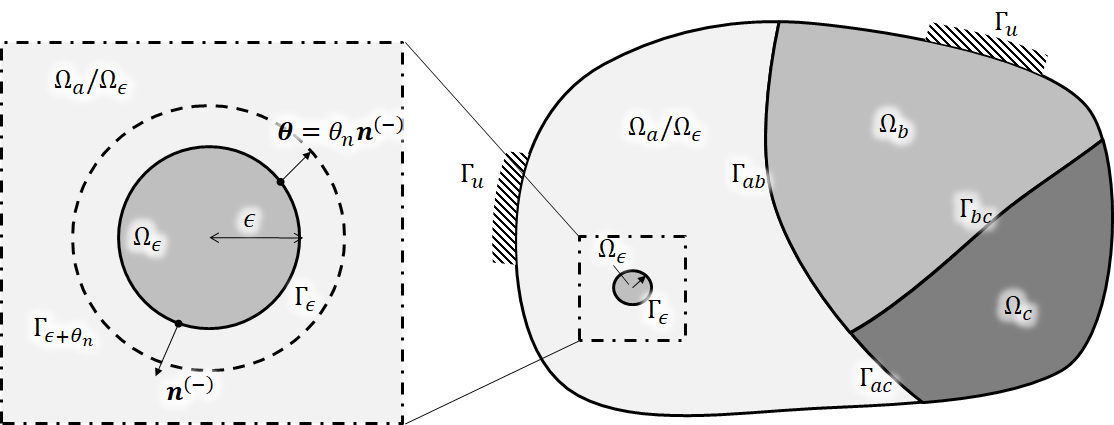
\includegraphics[width=13cm]{./figures/SDforTD.png}
		\caption{Topological derivative}
		\label{fig:TD}
	\end{center}
\end{figure}

$\bm{\theta}$を次式のように設定する
\begin{align}
	\bm{\theta}=&\theta_{n}\bm{n}^{(-)}	\hspace{1cm}\text{on}\hspace{0.3cm}\Gamma_{\epsilon}\\
	\bm{\theta}=&\bm{0}					\hspace{1.8cm}\text{on}\hspace{0.3cm}\Gamma/\Gamma_{\epsilon}
\end{align}
この時,固有値$\lambda$の形状微分は,\eqref{eq:shape_lambda}に
$\bm{u}=\bm{u}^{\epsilon},\lambda=\lambda^{\epsilon}$を代入することで以下のようになる.
\begin{align}
	&\hspace{0.5cm}D\lambda(\Omega_{p\{1\leq p\leq n\}})\cdot\bm{\theta}
	\nonumber
	\\
	=&\int_{\Gamma_\epsilon}(\theta_{n}n_{\gamma}^{(-)}n_{\gamma}^{(-)})
	\Bigr(u_{i,j}^{\epsilon(-)}C_{ijkl}^{b}u_{k,l}^{\epsilon(-)}
	-\lambda^{\epsilon}\rho^{b}u_{i}^{\epsilon(-)}u_{i}^{\epsilon(-)}\Bigl) d\Omega
	\nonumber
	\\
	&+\int_{\Gamma_\epsilon}(\theta_{n}n_{\gamma}^{(-)}n_{\gamma}^{(+)})
	\Bigr(u_{i,j}^{\epsilon(+)}C_{ijkl}^{a}u_{k,l}^{\epsilon(+)}
	-\lambda^{\epsilon}\rho^{a}u_{i}^{\epsilon(+)}u_{i}^{\epsilon(+)}\Bigl) d\Omega
	\nonumber
	\\
	&-\int_{\Gamma_{\epsilon}}(\theta_{n}n_{\gamma}^{(-)}n_{\gamma}^{(-)})
	\Bigr(C_{ijkl}^{b}u_{k,l}^{\epsilon(-)}n_{j}^{(-)}
	-C_{ijkl}^{a}u_{k,l}^{\epsilon(+)}n_{j}^{(+)}\Bigl)
	(u_{i,m}^{\epsilon(-)}n_{m}^{(-)}-u_{i,m}^{\epsilon(+)}n_{m}^{(-)}) d\Gamma
	\nonumber
	\\
	=&\theta_{n}\int_{\Gamma_\epsilon}
	\Bigr(u_{i,j}^{\epsilon(-)}C_{ijkl}^{b}u_{k,l}^{\epsilon(-)}
	-\lambda^{\epsilon}\rho^{b}u_{i}^{\epsilon(-)}u_{i}^{\epsilon(-)}\Bigl) d\Omega
	\nonumber
	\\
	&-\theta_{n}\int_{\Gamma_\epsilon}
	\Bigr(u_{i,j}^{\epsilon(+)}C_{ijkl}^{a}u_{k,l}^{\epsilon(+)}
	-\lambda^{\epsilon}\rho^{a}u_{i}^{\epsilon(+)}u_{i}^{\epsilon(+)}\Bigl) d\Omega
	\nonumber
	\\
	&-\theta_{n}\int_{\Gamma_{\epsilon}}
	\Bigr(C_{ijkl}^{b}u_{k,l}^{\epsilon(-)}n_{j}^{(-)}
	+C_{ijkl}^{a}u_{k,l}^{\epsilon(+)}n_{j}^{(-)}\Bigl)
	(u_{i,m}^{\epsilon(-)}n_{m}^{(-)}-u_{i,m}^{\epsilon(+)}n_{m}^{(-)}) d\Gamma
	\label{eq:SDForTD}
\end{align}

\begin{figure}[ht]
	\begin{center}
		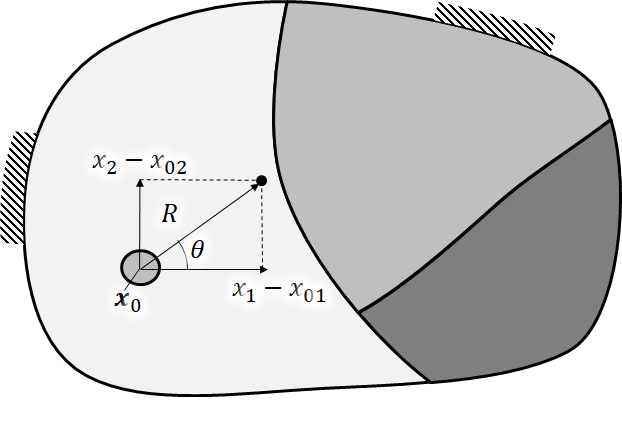
\includegraphics[height=5cm]{./figures/Rtheta.png}
		\caption{$(R,\theta)$ coordinate}
		\label{fig:Rtheta}
	\end{center}
\end{figure}
ここで,式\eqref{eq:w1InSol},\eqref{eq:w1OutSol}より,
\begin{align}
	\bm{u}^{\epsilon(-)}(\bm{x})=\bm{u}(\bm{z})
		+\epsilon\bm{\hat{w}}^{(I\hspace{-.15em}I-)}(\bm{\xi})+O(\epsilon^2)
	\nonumber
	\\
	\bm{u}^{\epsilon(+)}(\bm{x})=\bm{u}(\bm{x})
		+\epsilon\bm{\hat{w}}^{(I\hspace{-.15em}I+)}(\bm{\xi})+O(\epsilon^2)
\end{align}
\begin{align}
	\hat{w}_{\xi_{1}}^{(I\hspace{-.15em}I-)}(\bm{\xi})
	=&\hat{w}_{r}^{(I\hspace{-.15em}I-)}\cos(\theta)+\hat{w}_{\theta}^{(I\hspace{-.15em}I-)}\sin(\theta)
	\nonumber
	\\
	=&\frac{\mu^{a}\bigl(\kappa^{b}-1\bigr)(\kappa^{a}+1)}{2\bigl(\mu^{a}(\kappa^{b}-1)+2\mu^{b}\bigr)(\kappa^{a}-1)}
		\bigl\{u_{x_{1},x_{1}}(\bm{z})+u_{x_{2},x_{2}}(\bm{z})\bigr\}r\cos(\theta)
		\nonumber
		\\
		&+\frac{1}{2}\bigl\{u_{x_{1},x_{2}}(\bm{z})-u_{x_{2},x_{1}}(\bm{z})\bigr\}r\sin(\theta)
		\nonumber
		\\
		&+\frac{\mu^{a}\bigl(\kappa^{a}+1\bigr)}{2\bigl(\mu^{a}+\kappa^{a}\mu^{b}\bigr)}
		\bigl\{u_{x_{1},x_{1}}(\bm{z})-u_{x_{2},x_{2}}(\bm{z})\bigr\}r\cos(\theta)
		\nonumber
		\\
		&+\frac{\mu^{a}\bigl(\kappa^{a}+1\bigr)}{2\bigl(\mu^{a}+\kappa^{a}\mu^{b}\bigr)}
		\bigl\{u_{x_{1},x_{2}}(\bm{z})+u_{x_{2},x_{1}}(\bm{z})\bigr\}r\sin(\theta)
		\nonumber
	\\
	=&\frac{\mu^{a}\bigl(\kappa^{b}-1\bigr)(\kappa^{a}+1)}{2\bigl(\mu^{a}(\kappa^{b}-1)+2\mu^{b}\bigr)(\kappa^{a}-1)}
		\bigl\{u_{x_{1},x_{1}}(\bm{z})+u_{x_{2},x_{2}}(\bm{z})\bigr\}\xi_{1}
		\nonumber
		\\
		&+\frac{1}{2}\bigl\{u_{x_{1},x_{2}}(\bm{z})-u_{x_{2},x_{1}}(\bm{z})\bigr\}\xi_{2}
		\nonumber
		\\
		&+\frac{\mu^{a}\bigl(\kappa^{a}+1\bigr)}{2\bigl(\mu^{a}+\kappa^{a}\mu^{b}\bigr)}
		\bigl\{u_{x_{1},x_{1}}(\bm{z})-u_{x_{2},x_{2}}(\bm{z})\bigr\}\xi_{1}
		\nonumber
		\\
		&+\frac{\mu^{a}\bigl(\kappa^{a}+1\bigr)}{2\bigl(\mu^{a}+\kappa^{a}\mu^{b}\bigr)}
		\bigl\{u_{x_{1},x_{2}}(\bm{z})+u_{x_{2},x_{1}}(\bm{z})\bigr\}\xi_{2}
	\\
	\hat{w}_{\xi_{2}}^{(I\hspace{-.15em}I-)}(\bm{\xi})
	=&\hat{w}_{r}^{(I\hspace{-.15em}I-)}\sin(\theta)+\hat{w}_{\theta}^{(I\hspace{-.15em}I-)}\cos(\theta)
	\nonumber
	\\
	=&\frac{\mu^{a}\bigl(\kappa^{b}-1\bigr)(\kappa^{a}+1)}{2\bigl(\mu^{a}(\kappa^{b}-1)+2\mu^{b}\bigr)(\kappa^{a}-1)}
			\bigl\{u_{x_{1},x_{1}}(\bm{z})+u_{x_{2},x_{2}}(\bm{z})\bigr\}\xi_{2}
		\nonumber
		\\
		&-\frac{1}{2}\bigl\{u_{x_{1},x_{2}}(\bm{z})-u_{x_{2},x_{1}}(\bm{z})\bigr\}\xi_{1}
		\nonumber
		\\
		&-\frac{\mu^{a}\bigl(\kappa^{a}+1\bigr)}{2\bigl(\mu^{a}+\kappa^{a}\mu^{b}\bigr)}
		\bigl\{u_{x_{1},x_{1}}(\bm{z})-u_{x_{2},x_{2}}(\bm{z})\bigr\}\xi_{2}
		\nonumber
		\\
		&+\frac{\mu^{a}\bigl(\kappa^{a}+1\bigr)}{2\bigl(\mu^{a}+\kappa^{a}\mu^{b}\bigr)}
		\bigl\{u_{x_{1},x_{2}}(\bm{z})+u_{x_{2},x_{1}}(\bm{z})\bigr\}\xi_{1}
\end{align}
\begin{align}
	\hat{w}_{\xi_{1}}^{(I\hspace{-.15em}I+)}(\bm{\xi})
	=&\hat{w}_{r}^{(I\hspace{-.15em}I-)}\cos(\theta)+\hat{w}_{\theta}^{(I\hspace{-.15em}I-)}\sin(\theta)
	\nonumber
	\\
	=&\frac{\mu^{a}\bigl(\kappa^{b}-1\bigr)-\mu^{b}\bigl(\kappa^{a}-1\bigr)}
			{\bigl(\mu^{a}(\kappa^{b}-1)+2\mu^{b}\bigr)(\kappa^{a}-1)}
			\bigl\{u_{x_{1},x_{1}}(\bm{z})+u_{x_{2},x_{2}}(\bm{z})\bigr\}r^{-1}\cos(\theta)
		\nonumber
		\\
		&+\frac{\mu^{a}-\mu^{b}}{2\bigl(\mu^{a}+\kappa^{a}\mu^{b}\bigr)}
		\bigl\{u_{x_{1},x_{1}}(\bm{z})-u_{x_{2},x_{2}}(\bm{z})\bigr\}
		\bigl\{(\kappa^{a}+1)r^{-1}-r^{-3}\bigr\}\cos(\theta)
		\nonumber
		\\
		&+\frac{\mu^{a}-\mu^{b}}{2\bigl(\mu^{a}+\kappa^{a}\mu^{b}\bigr)}
		\bigl\{u_{x_{1},x_{2}}(\bm{z})+u_{x_{2},x_{1}}(\bm{z})\bigr\}
		\bigl\{(\kappa^{a}+1)r^{-1}-r^{-3}\bigr\}\sin(\theta)
		\nonumber
		\\
	=&\frac{\mu^{a}\bigl(\kappa^{b}-1\bigr)-\mu^{b}\bigl(\kappa^{a}-1\bigr)}
			{\bigl(\mu^{a}(\kappa^{b}-1)+2\mu^{b}\bigr)(\kappa^{a}-1)}
			\bigl\{u_{x_{1},x_{1}}(\bm{z})+u_{x_{2},x_{2}}(\bm{z})\bigr\}|\bm{\xi}|^{-2}\xi_{1}
		\nonumber
		\\
		&+\frac{\mu^{a}-\mu^{b}}{2\bigl(\mu^{a}+\kappa^{a}\mu^{b}\bigr)}
		\bigl\{u_{x_{1},x_{1}}(\bm{z})-u_{x_{2},x_{2}}(\bm{z})\bigr\}
		\bigl\{(\kappa^{a}+1)|\bm{\xi}|^{-2}-|\bm{\xi}|^{-4}\bigr\}\xi_{1}
		\nonumber
		\\
		&+\frac{\mu^{a}-\mu^{b}}{2\bigl(\mu^{a}+\kappa^{a}\mu^{b}\bigr)}
		\bigl\{u_{x_{1},x_{2}}(\bm{z})+u_{x_{2},x_{1}}(\bm{z})\bigr\}
		\bigl\{(\kappa^{a}+1)|\bm{\xi}|^{-2}-|\bm{\xi}|^{-4}\bigr\}\xi_{2}
	\\
	\hat{w}_{\xi_{2}}^{(I\hspace{-.15em}I-)}(\bm{\xi})=&
			\hat{w}_{r}^{(I\hspace{-.15em}I-)}\sin(\theta)+\hat{w}_{\theta}^{(I\hspace{-.15em}I-)}\cos(\theta)
		\nonumber
		\\
		=&\frac{\mu^{a}\bigl(\kappa^{b}-1\bigr)-\mu^{b}\bigl(\kappa^{a}-1\bigr)}
			{\bigl(\mu^{a}(\kappa^{b}-1)+2\mu^{b}\bigr)(\kappa^{a}-1)}
			\bigl\{u_{x_{1},x_{1}}(\bm{z})+u_{x_{2},x_{2}}(\bm{z})\bigr\}|\bm{\xi}|^{-2}\xi_{2}
		\nonumber
		\\
		&-\frac{\mu^{a}-\mu^{b}}{2\bigl(\mu^{a}+\kappa^{a}\mu^{b}\bigr)}
		\bigl\{u_{x_{1},x_{1}}(\bm{z})-u_{x_{2},x_{2}}(\bm{z})\bigr\}
		\bigl\{(\kappa^{a}+1)|\bm{\xi}|^{-2}-|\bm{\xi}|^{-4}\bigr\}\xi_{2}
		\nonumber
		\\
		&+\frac{\mu^{a}-\mu^{b}}{2\bigl(\mu^{a}+\kappa^{a}\mu^{b}\bigr)}
		\bigl\{u_{x_{1},x_{2}}(\bm{z})+u_{x_{2},x_{1}}(\bm{z})\bigr\}
		\bigl\{(\kappa^{a}+1)|\bm{\xi}|^{-2}-|\bm{\xi}|^{-4}\bigr\}\xi_{1}
\end{align}
ゆえに,$\dsp\frac{\partial}{\partial x_{i}}=\frac{1}{\epsilon}\frac{\partial}{\partial \xi_{i}}$より,
\begin{align}
	\frac{\partial u_{i}^{\epsilon(-)}}{\partial x_{j}}(\bm{x})=
		\frac{\partial\hat{w}_{i}^{(I\hspace{-.15em}I-)}}{\partial \xi_{j}}(\bm{\xi})+O(\epsilon)
	\nonumber
	\\
	\frac{\partial u_{i}^{\epsilon(+)}}{\partial x_{j}}(\bm{x})
	=\frac{\partial u_{i}}{\partial x_{j}}(\bm{x})
		+\frac{\partial\hat{w}_{i}^{(I\hspace{-.15em}I+)}}{\partial \xi_{j}}(\bm{\xi})+O(\epsilon)
\end{align}
となる.
\begin{align}
	x_{1}-z_{1}=R\cos(\theta)
	\nonumber
	\\
	x_{2}-z_{2}=R\sin(\theta)
	\label{eq:xyToRTh}
\end{align}
と座標変換すると$R,\theta$方向の変位は以下のようになる.
\begin{align}
	u_{R}^{\epsilon(-)}(r,\theta)=&\hat{w}_{r}^{(I-)}(\theta)
	+\epsilon\hat{w}_{r}^{(I\hspace{-.15em}I-)}(r,\theta)+O(\epsilon^2)
	\nonumber
	\\
	u_{\theta}^{\epsilon(-)}(r,\theta)=&\hat{w}_{\theta}^{(I-)}(\theta)
	+\epsilon\hat{w}_{\theta}^{(I\hspace{-.15em}I-)}(r,\theta)+O(\epsilon^2)
	\nonumber
	\\
	u_{R}^{\epsilon(+)}(R,r,\theta)=&u_{x_{1}}(\bm{x})\cos(\theta)+u_{x_{2}}(\bm{x})\sin(\theta)
	+\epsilon\hat{w}_{r}^{(I\hspace{-.15em}I+)}(r,\theta)+O(\epsilon^2)
	\nonumber
	\\
	u_{\theta}^{\epsilon(+)}(R,r,\theta)=&-u_{x_{1}}(\bm{x})\sin(\theta)+u_{x_{2}}(\bm{x})\cos(\theta)
	+\epsilon\hat{w}_{\theta}^{(I\hspace{-.15em}I+)}(r,\theta)+O(\epsilon^2)
	\label{eq:SDForTD}
\end{align}
$R=\epsilon r$の関係から,
\begin{align}
	\frac{\partial}{\partial R}=\frac{1}{\epsilon}\frac{\partial}{\partial r}
	\label{eq:RTor}
\end{align}
であることに注意して歪みや応力を計算すると以下のようになる.
\begin{align}
	e_{RR}^{\epsilon(-)}
		=&\frac{\partial u_{R}^{\epsilon(-)}}{\partial R}
		\nonumber
		\\
		=&\epsilon\frac{1}{\epsilon}\frac{\partial\hat{w}_{r}^{(I\hspace{-.15em}I-)}}{\partial r}(r,\theta)+O(\epsilon)
		\nonumber
		\\
		=&\frac{\partial\hat{w}_{r}^{(I\hspace{-.15em}I-)}}{\partial r}(r,\theta)+O(\epsilon)
		\label{eq:eRRInEps}
\end{align}
\begin{align}
	e_{R\theta}^{\epsilon(-)}
		=&\frac{1}{2}\Bigl( \frac{1}{R}\frac{\partial u_{R}^{\epsilon(-)}}{\partial \theta}
			+\frac{\partial u_{\theta}^{\epsilon(-)}}{\partial R}-\frac{u_{\theta}^{\epsilon(-)}}{R}\Bigr)
		\nonumber
		\\
		=&\frac{1}{2}\Bigl( \frac{1}{\epsilon r}\frac{\partial \hat{w}_{r}^{(I-)}}{\partial \theta}
			-\frac{\hat{w}_{\theta}^{(I-)}}{\epsilon r}
			+\frac{1}{r}\frac{\partial \hat{w}_{r}^{(I\hspace{-.15em}I-)}}{\partial \theta}
			+\frac{\partial \hat{w}_{\theta}^{(I\hspace{-.15em}I-)}}{\partial r}
			-\frac{\hat{w}_{\theta}^{(I\hspace{-.15em}I-)}}{r}\Bigr)+O(\epsilon)
\end{align}
\begin{align}
	e_{\theta\theta}^{\epsilon(-)}
		=&\frac{1}{R}\frac{\partial u_{\theta}^{\epsilon(-)}}{\partial \theta}
			+\frac{u_{R}^{\epsilon(-)}}{R}
		\nonumber
		\\
		=&\frac{1}{r}\frac{\partial \hat{w}_{\theta}^{(I\hspace{-.15em}I-)}}{\partial \theta}
			+\frac{\hat{w}_{r}^{(I\hspace{-.15em}I-)}}{r}+O(\epsilon)
\end{align}

また,
\begin{align}
	e_{RR}
		=&e_{x_{1}x_{1}}\cos^2(\theta)+e_{x_{2}x_{2}}\sin^2(\theta)+2e_{x_{1}x_{2}}\sin(\theta)\cos(\theta)
		\nonumber
		\\
	e_{\theta\theta}
		=&e_{x_{1}x_{1}}\sin^2(\theta)+e_{x_{2}x_{2}}\cos^2(\theta)-2e_{x_{1}x_{2}}\sin(\theta)\cos(\theta)
		\nonumber
		\\
	e_{r\theta}
		=&\bigl(e_{x_{2}x_{2}}-e_{x_{1}x_{1}}\bigr)\sin(\theta)\cos(\theta)+e_{x_{1}x_{2}}\bigl(\cos^2(\theta)-\sin^2(\theta)\bigr)
\end{align}
より,
\begin{align}
	e_{RR}^{\epsilon(+)}
		=&\frac{\partial u_{R}^{\epsilon(+)}}{\partial R}
		\nonumber
		\\
		=&\frac{1}{2}\Bigl\{ \frac{\partial u_{x_{1}}}{\partial x_{1}}(\bm{x})
			+\frac{\partial u_{x_{2}}}{\partial x_{2}}(\bm{x})\Bigr\}
		+\frac{1}{2}\Bigl\{ \frac{\partial u_{x_{1}}}{\partial x_{1}}(\bm{x})
			-\frac{\partial u_{x_{2}}}{\partial x_{2}}(\bm{x})\Bigr\}\cos(2\theta)
		\nonumber
		\\
		&+\frac{1}{2}\Bigl\{ \frac{\partial u_{x_{1}}}{\partial x_{2}}(\bm{x})
			+\frac{\partial u_{x_{2}}}{\partial x_{1}}(\bm{x})\Bigr\}\sin(2\theta)
		+\frac{\partial\hat{w}_{r}^{(I\hspace{-.15em}I+)}}{\partial r}(r,\theta)+O(\epsilon)
		\label{eq:eRROutEps}
\end{align}
\begin{align}
	e_{R\theta}^{\epsilon(+)}
		=&\frac{1}{2}\Bigl( \frac{1}{R}\frac{\partial u_{R}^{\epsilon(+)}}{\partial \theta}
			+\frac{\partial u_{\theta}^{\epsilon(+)}}{\partial R}-\frac{u_{\theta}^{\epsilon(+)}}{R}\Bigr)
		\nonumber
		\\
		=&-\frac{1}{2}\Bigl\{ \frac{\partial u_{x_{1}}}{\partial x_{1}}(\bm{x})
			-\frac{\partial u_{x_{2}}}{\partial x_{2}}(\bm{x})\Bigr\}\sin(2\theta)
		+\frac{1}{2}\Bigl\{ \frac{\partial u_{x_{1}}}{\partial x_{2}}(\bm{x})
			+\frac{\partial u_{x_{2}}}{\partial x_{1}}(\bm{x})\Bigr\}\cos(2\theta)
			\nonumber
			\\
		&+\frac{1}{2}\Bigl( \frac{1}{r}\frac{\partial \hat{w}_{r}^{(I\hspace{-.15em}I+)}}{\partial \theta}
			+\frac{\partial \hat{w}_{\theta}^{(I\hspace{-.15em}I+)}}{\partial r}
			-\frac{\hat{w}_{\theta}^{(I\hspace{-.15em}I+)}}{r}\Bigr)+O(\epsilon)
\end{align}
\begin{align}
	e_{\theta\theta}^{\epsilon(+)}
		=&\frac{1}{R}\frac{\partial u_{\theta}^{\epsilon(+)}}{\partial \theta}
			+\frac{u_{R}^{\epsilon(+)}}{R}
		\nonumber
		\\
		=&\frac{1}{2}\Bigl\{ \frac{\partial u_{x_{1}}}{\partial x_{1}}(\bm{x})
			+\frac{\partial u_{x_{2}}}{\partial x_{2}}(\bm{x})\Bigr\}
		-\frac{1}{2}\Bigl\{ \frac{\partial u_{x_{1}}}{\partial x_{1}}(\bm{x})
			-\frac{\partial u_{x_{2}}}{\partial x_{2}}(\bm{x})\Bigr\}\cos(2\theta)
		\nonumber
		\\
		&-\frac{1}{2}\Bigl\{ \frac{\partial u_{x_{1}}}{\partial x_{2}}(\bm{x})
			+\frac{\partial u_{x_{2}}}{\partial x_{1}}(\bm{x})\Bigr\}\sin(2\theta)
		+\frac{1}{r}\frac{\partial \hat{w}_{\theta}^{(I\hspace{-.15em}I+)}}{\partial \theta}
			+\frac{\hat{w}_{r}^{(I\hspace{-.15em}I+)}}{r}+O(\epsilon)
	\label{eq:eThThOutEps}
\end{align}

$\Gamma_\epsilon$上での歪みは以下のようになる.
\begin{align}
	e_{RR}^{\epsilon(-)}
	=&\frac{\mu^{a}(\kappa^{b}-1)(\kappa^{a}+1)}{2\bigl(\mu^{a}(\kappa^{b}-1)+2\mu^{b}\bigr)(\kappa^{a}-1)}
	\bigl\{u_{x_{1},x_{1}}(\bm{x_{0}})+u_{x_{2},x_{2}}(\bm{x_{0}})\bigr\}
	\nonumber
	\\
	&+\frac{\mu^{a}\bigl(\kappa^{a}+1\bigr)}{2\bigl(\mu^{a}+\kappa^{a}\mu^{b}\bigr)}
	\bigl\{u_{x_{1},x_{1}}(\bm{x_{0}})-u_{x_{2},x_{2}}(\bm{x_{0}})\bigr\}\cos(2\theta)
	\nonumber
	\\
	&+\frac{\mu^{a}\bigl(\kappa^{a}+1\bigr)}{2\bigl(\mu^{a}+\kappa^{a}\mu^{b}\bigr)}
	\bigl\{u_{x_{1},x_{2}}(\bm{x_{0}})+u_{x_{2},x_{1}}(\bm{x_{0}})\bigr\}\sin(2\theta)
	\label{eq:eRRInEpsSol}
\end{align}
\begin{align}
	e_{R\theta}^{\epsilon(-)}
	=&-\frac{\mu^{a}\bigl(\kappa^{a}+1\bigr)}{2\bigl(\mu^{a}+\kappa^{a}\mu^{b}\bigr)}
	\bigl\{u_{x_{1},x_{1}}(\bm{x_{0}})-u_{x_{2},x_{2}}(\bm{x_{0}})\bigr\}\sin(2\theta)
	\nonumber
	\\
	&+\frac{\mu^{a}\bigl(\kappa^{a}+1\bigr)}{2\bigl(\mu^{a}+\kappa^{a}\mu^{b}\bigr)}
	\bigl\{u_{x_{1},x_{2}}(\bm{x_{0}})+u_{x_{2},x_{1}}(\bm{x_{0}})\bigr\}\cos(2\theta)
	\label{eq:eRThInEpsSol}
\end{align}
\begin{align}
	e_{\theta\theta}^{\epsilon(-)}
	=&\frac{\mu^{a}(\kappa^{b}-1)(\kappa^{a}+1)}{2\bigl(\mu^{a}(\kappa^{b}-1)+2\mu^{b}\bigr)}
	\bigl\{u_{x_{1},x_{1}}(\bm{x_{0}})+u_{x_{2},x_{2}}(\bm{x_{0}})\bigr\}
	\nonumber
	\\
	&-\frac{\mu^{a}\bigl(\kappa^{a}+1\bigr)}{2\bigl(\mu^{a}+\kappa^{a}\mu^{b}\bigr)}
	\bigl\{u_{x_{1},x_{1}}(\bm{x_{0}})-u_{x_{2},x_{2}}(\bm{x_{0}})\bigr\}\cos(2\theta)
	\nonumber
	\\
	&-\frac{\mu^{a}\bigl(\kappa^{a}+1\bigr)}{2\bigl(\mu^{a}+\kappa^{a}\mu^{b}\bigr)}
	\bigl\{u_{x_{1},x_{2}}(\bm{x_{0}})+u_{x_{2},x_{1}}(\bm{x_{0}})\bigr\}\sin(2\theta)
	\label{eq:eThThInEpsSol}
\end{align}

%外側の歪み
\begin{align}
	\hat{e}_{rr}^{(I\hspace{-.15em}I+)} =
	&-\frac{ \mu^{a}\bigl(\kappa^{b}-1\bigr)-\mu^{b}\bigl(\kappa^{a}-1\bigr) }
	{\bigl(\mu^{a}(\kappa^{b}-1)+2\mu^{b}\bigr)(\kappa^{a}-1)}
	\bigl\{u_{x_{1},x_{1}}(\bm{x_{0}})+u_{x_{2},x_{2}}(\bm{x_{0}})\bigr\}
	\nonumber
	\\
	&-\frac{\bigl(\mu^{a}-\mu^{b}\bigr)\bigl(\kappa^{a}-2\bigr)}{2\bigl(\mu^{a}+\kappa^{a}\mu^{b}\bigr)}
	\bigl\{u_{x_{1},x_{1}}(\bm{x_{0}})-u_{x_{2},x_{2}}(\bm{x_{0}})\bigr\}\cos(2\theta)
	\nonumber
	\\
	&-\frac{\bigl(\mu^{a}-\mu^{b}\bigr)\bigl(\kappa^{a}-2\bigr)}{2\bigl(\mu^{a}+\kappa^{a}\mu^{b}\bigr)}
	\bigl\{u_{x_{1},x_{2}}(\bm{x_{0}})+u_{x_{2},x_{1}}(\bm{x_{0}})\bigr\}\sin(2\theta)
	\label{eq:eRROut2Sol}
\end{align}
\begin{align}
	\hat{e}_{r\theta}^{(I\hspace{-.15em}I+)} =
	&\frac{\bigl(\mu^{a}-\mu^{b}\bigr)}{2\bigl(\mu^{a}+\kappa^{a}\mu^{b}\bigr)}
	\bigl\{u_{x_{1},x_{1}}(\bm{x_{0}})-u_{x_{2},x_{2}}(\bm{x_{0}})\bigr\}\sin(2\theta)
	\nonumber
	\\
	&-\frac{\bigl(\mu^{a}-\mu^{b}\bigr)}{2\bigl(\mu^{a}+\kappa^{a}\mu^{b}\bigr)}
	\bigl\{u_{x_{1},x_{2}}(\bm{x_{0}})+u_{x_{2},x_{1}}(\bm{x_{0}})\bigr\}\cos(2\theta)
	\label{eq:eRThOut2Sol}
\end{align}
\begin{align}
	\hat{e}_{\theta\theta}^{(I\hspace{-.15em}I+)} =
	&\frac{ \mu^{a}\bigl(\kappa^{b}-1\bigr)-\mu^{b}\bigl(\kappa^{a}-1\bigr) }
	{\bigl(\mu^{a}(\kappa^{b}-1)+2\mu^{b}\bigr)(\kappa^{a}-1)}
	\bigl\{u_{x_{1},x_{1}}(\bm{x_{0}})+u_{x_{2},x_{2}}(\bm{x_{0}})\bigr\}
	\nonumber
	\\
	&-\frac{\bigl(\mu^{a}-\mu^{b}\bigr)\kappa^{a}}{2\bigl(\mu^{a}+\kappa^{a}\mu^{b}\bigr)}
	\bigl\{u_{x_{1},x_{1}}(\bm{x_{0}})-u_{x_{2},x_{2}}(\bm{x_{0}})\bigr\}\cos(2\theta)
	\nonumber
	\\
	&-\frac{\bigl(\mu^{a}-\mu^{b}\bigr)\kappa^{a}}{2\bigl(\mu^{a}+\kappa^{a}\mu^{b}\bigr)}
	\bigl\{u_{x_{1},x_{2}}(\bm{x_{0}})+u_{x_{2},x_{1}}(\bm{x_{0}})\bigr\}\sin(2\theta)
	\label{eq:eThThOut2Sol}
\end{align}

%外側の歪みの合計
\begin{align}
	e_{RR}^{\epsilon(+)}
	=&\frac{ \mu^{a}\bigl(\kappa^{b}-1\bigr)\bigl(\kappa^{a}-3\bigr)+4\mu^{b}\bigl(\kappa^{a}-1\bigr) }
		{2\bigl(\mu^{a}(\kappa^{b}-1)+2\mu^{b}\bigr)(\kappa^{a}-1)}
	\bigl\{u_{x_{1},x_{1}}(\bm{x_{0}})+u_{x_{2},x_{2}}(\bm{x_{0}})\bigr\}
	\nonumber
	\\
	&+\frac{\mu^{a}\bigl(3-\kappa^{a}\bigr)+2\mu^{b}\bigl(\kappa^{a}-1\bigr)}{2\bigl(\mu^{a}+\kappa^{a}\mu^{b}\bigr)}
	\bigl\{u_{x_{1},x_{1}}(\bm{x_{0}})-u_{x_{2},x_{2}}(\bm{x_{0}})\bigr\}\cos(2\theta)
	\nonumber
	\\
	&+\frac{\mu^{a}\bigl(3-\kappa^{a}\bigr)+2\mu^{b}\bigl(\kappa^{a}-1\bigr)}{2\bigl(\mu^{a}+\kappa^{a}\mu^{b}\bigr)}
	\bigl\{u_{x_{1},x_{2}}(\bm{x_{0}})+u_{x_{2},x_{1}}(\bm{x_{0}})\bigr\}\sin(2\theta)
	\label{eq:eRROutEpsSol}
\end{align}
\begin{align}
	e_{R\theta}^{\epsilon(+)}
	=&-\frac{\mu^{b}\bigl(\kappa^{a}+1\bigr)}{2(\mu^{a}+\kappa^{a}\mu^{b})}
	\bigl\{u_{x_{1},x_{1}}(\bm{x_{0}})-u_{x_{2},x_{2}}(\bm{x_{0}})\bigr\}\sin(2\theta)
	\nonumber
	\\
	&+\frac{\mu^{b}\bigl(\kappa^{a}+1\bigr)}{\mu^{a}+\kappa^{a}\mu^{b}}
	\bigl\{u_{x_{1},x_{2}}(\bm{x_{0}})+u_{x_{2},x_{1}}(\bm{x_{0}})\bigr\}\cos(2\theta)
	\label{eq:eRThOutEpsSol}
\end{align}
\begin{align}
	e_{\theta\theta}^{\epsilon(+)}
	=&\frac{\mu^{a}(\kappa^{b}-1)(\kappa^{a}+1)}
	{2\bigl(\mu^{a}(\kappa^{b}-1)+2\mu^{b}\bigr)(\kappa^{a}-1)}
	\bigl\{u_{x_{1},x_{1}}(\bm{x_{0}})+u_{x_{2},x_{2}}(\bm{x_{0}})\bigr\}
	\nonumber
	\\
	&-\frac{\mu^{a}\bigl(\kappa^{a}+1\bigr)}{2\bigl(\mu^{a}+\kappa^{a}\mu^{b}\bigr)}
	\bigl\{u_{x_{1},x_{1}}(\bm{x_{0}})-u_{x_{2},x_{2}}(\bm{x_{0}})\bigr\}\cos(2\theta)
	\nonumber
	\\
	&-\frac{\mu^{a}\bigl(\kappa^{a}+1\bigr)}{2\bigl(\mu^{a}+\kappa^{a}\mu^{b}\bigr)}
	\bigl\{u_{x_{1},x_{2}}(\bm{x_{0}})+u_{x_{2},x_{1}}(\bm{x_{0}})\bigr\}\sin(2\theta)
	\label{eq:eThThOutEpsSol}
\end{align}
歪みと応力の関係\eqref{eq:Constitute2}より,応力は以下のようになる.
\begin{align}
	\sigma_{RR}
	=&\frac{\kappa+1}{\kappa-1}\mu e_{RR}^{}+\frac{3-\kappa}{\kappa-1}\mu e_{\theta\theta}^{}
	\nonumber
	\\
	\sigma_{\theta\theta}
	=&\frac{\kappa+1}{\kappa-1}\mu e_{\theta\theta}^{}+\frac{3-\kappa}{\kappa-1}\mu e_{RR}^{}
	\nonumber
	\\
	\sigma_{R\theta}=&2\mu e_{R\theta}^{}
	\label{eq:Constitute2}
\end{align}

\begin{align}
	\sigma_{RR}^{\epsilon(-)} =
	&\frac{2\mu^{a}\mu^{b}(\kappa^{a}+1)}{\bigl(\mu^{a}(\kappa^{b}-1)+2\mu^{b}\bigr)(\kappa^{a}-1)}
	\bigl\{u_{x_{1},x_{1}}(\bm{x_{0}})+u_{x_{2},x_{2}}(\bm{x_{0}})\bigr\}
	\nonumber
	\\
	&+\frac{\mu^{a}\mu^{b}\bigl(\kappa^{a}+1\bigr)}{\mu^{a}+\kappa^{a}\mu^{b}}
	\bigl\{u_{x_{1},x_{1}}(\bm{x_{0}})-u_{x_{2},x_{2}}(\bm{x_{0}})\bigr\}\cos(2\theta)
	\nonumber
	\\
	&+\frac{\mu^{a}\mu^{b}\bigl(\kappa^{a}+1\bigr)}{\mu^{a}+\kappa^{a}\mu^{b}}
	\bigl\{u_{x_{1},x_{2}}(\bm{x_{0}})+u_{x_{2},x_{1}}(\bm{x_{0}})\bigr\}\sin(2\theta)
	\label{eq:SigmaRRInEpsSol}
\end{align}
\begin{align}
	\sigma_{R\theta}^{\epsilon(-)} =
	&-\frac{\mu^{a}\mu^{b}\bigl(\kappa^{a}+1\bigr)}{\mu^{a}+\kappa^{a}\mu^{b}}
	\bigl\{u_{x_{1},x_{1}}(\bm{x_{0}})-u_{x_{2},x_{2}}(\bm{x_{0}})\bigr\}\sin(2\theta)
	\nonumber
	\\
	&+\frac{\mu^{a}\mu^{b}\bigl(\kappa^{a}+1\bigr)}{\mu^{a}+\kappa^{a}\mu^{b}}
	\bigl\{u_{x_{1},x_{2}}(\bm{x_{0}})+u_{x_{2},x_{1}}(\bm{x_{0}})\bigr\}\cos(2\theta)
	\label{eq:SigmaRThInEpsSol}
\end{align}
\begin{align}
	\sigma_{\theta\theta}^{\epsilon(-)} =
	&\frac{2\mu^{a}\mu^{b}(\kappa^{a}+1)}{\bigl(\mu^{a}(\kappa^{b}-1)+2\mu^{b}\bigr)(\kappa^{a}-1)}
	\bigl\{u_{x_{1},x_{1}}(\bm{x_{0}})+u_{x_{2},x_{2}}(\bm{x_{0}})\bigr\}
	\nonumber
	\\
	&-\frac{\mu^{a}\mu^{b}\bigl(\kappa^{a}+1\bigr)}{\mu^{a}+\kappa^{a}\mu^{b}}
	\bigl\{u_{x_{1},x_{1}}(\bm{x_{0}})-u_{x_{2},x_{2}}(\bm{x_{0}})\bigr\}\cos(2\theta)
	\nonumber
	\\
	&-\frac{\mu^{a}\mu^{b}\bigl(\kappa^{a}+1\bigr)}{\mu^{a}+\kappa^{a}\mu^{b}}
	\bigl\{u_{x_{1},x_{2}}(\bm{x_{0}})+u_{x_{2},x_{1}}(\bm{x_{0}})\bigr\}\sin(2\theta)
	\label{eq:SigmaThThInEpsSol}
\end{align}

%外側の応力
\begin{align}
	\hat{\sigma}_{rr}^{(I\hspace{-.15em}I+)} =
	&-\frac{2\mu^{a}\bigl\{ \mu^{a}\bigl(\kappa^{b}-1\bigr)-\mu^{b}\bigl(\kappa^{a}-1\bigr)\bigr\}}
	{\bigl(\mu^{a}(\kappa^{b}-1)+2\mu^{b}\bigr)(\kappa^{a}-1)}
	\bigl\{u_{x_{1},x_{1}}(\bm{x_{0}})+u_{x_{2},x_{2}}(\bm{x_{0}})\bigr\}
	\nonumber
	\\
	&-\frac{\mu^{a}\bigl(\mu^{a}-\mu^{b}\bigr)}{\mu^{a}+\kappa^{a}\mu^{b}}
	\bigl\{u_{x_{1},x_{1}}(\bm{x_{0}})-u_{x_{2},x_{2}}(\bm{x_{0}})\bigr\}\cos(2\theta)
	\nonumber
	\\
	&-\frac{\mu^{a}\bigl(\mu^{a}-\mu^{b}\bigr)}{\mu^{a}+\kappa^{a}\mu^{b}}
	\bigl\{u_{x_{1},x_{2}}(\bm{x_{0}})+u_{x_{2},x_{1}}(\bm{x_{0}})\bigr\}r^{-2}\sin(2\theta)
	\label{eq:SigmaRROut2Sol}
\end{align}
\begin{align}
	\hat{\sigma}_{r\theta}^{(I\hspace{-.15em}I+)} =
	&\frac{\mu^{a}\bigl(\mu^{a}-\mu^{b}\bigr)}{\mu^{a}+\kappa^{a}\mu^{b}}
	\bigl\{u_{x_{1},x_{1}}(\bm{x_{0}})-u_{x_{2},x_{2}}(\bm{x_{0}})\bigr\}\sin(2\theta)
	\nonumber
	\\
	&-\frac{\mu^{a}\bigl(\mu^{a}-\mu^{b}\bigr)}{\mu^{a}+\kappa^{a}\mu^{b}}
	\bigl\{u_{x_{1},x_{2}}(\bm{x_{0}})+u_{x_{2},x_{1}}(\bm{x_{0}})\bigr\}\cos(2\theta)
	\label{eq:SigmaRThOut2Sol}
\end{align}
\begin{align}
	\hat{\sigma}_{\theta\theta}^{(I\hspace{-.15em}I+)} =
	&\frac{2\mu^{a}\bigl\{ \mu^{a}\bigl(\kappa^{b}-1\bigr)-\mu^{b}\bigl(\kappa^{a}-1\bigr)\bigr\}}
	{\bigl(\mu^{a}(\kappa^{b}-1)+2\mu^{b}\bigr)(\kappa^{a}-1)}
	\bigl\{u_{x_{1},x_{1}}(\bm{x_{0}})+u_{x_{2},x_{2}}(\bm{x_{0}})\bigr\}
	\nonumber
	\\
	&-\frac{3\mu^{a}\bigl(\mu^{a}-\mu^{b}\bigr)}{\mu^{a}+\kappa^{a}\mu^{b}}
	\bigl\{u_{x_{1},x_{1}}(\bm{x_{0}})-u_{x_{2},x_{2}}(\bm{x_{0}})\bigr\}\cos(2\theta)
	\nonumber
	\\
	&-\frac{3\mu^{a}\bigl(\mu^{a}-\mu^{b}\bigr)}{\mu^{a}+\kappa^{a}\mu^{b}}
	\bigl\{u_{x_{1},x_{2}}(\bm{x_{0}})+u_{x_{2},x_{1}}(\bm{x_{0}})\bigr\}\sin(2\theta)
	\label{eq:SigmaThThOut2Sol}
\end{align}

%元の応力の合計
\begin{align}
	\sigma_{RR}^{(+)}
	=&\frac{ 2\mu^{a}}{\kappa^{a}-1}
	\bigl\{u_{x_{1},x_{1}}(\bm{x_{0}})+u_{x_{2},x_{2}}(\bm{x_{0}})\bigr\}
	\nonumber
	\\
	&+\mu^{a}
	\bigl\{u_{x_{1},x_{1}}(\bm{x_{0}})-u_{x_{2},x_{2}}(\bm{x_{0}})\bigr\}\cos(2\theta)
	\nonumber
	\\
	&+\mu^{a}
	\bigl\{u_{x_{1},x_{2}}(\bm{x_{0}})+u_{x_{2},x_{1}}(\bm{x_{0}})\bigr\}\sin(2\theta)
	\label{eq:eRROutEpsSol}
\end{align}
\begin{align}
	\sigma_{R\theta}^{(+)}
	=&-\mu^{a}
	\bigl\{u_{x_{1},x_{1}}(\bm{x_{0}})-u_{x_{2},x_{2}}(\bm{x_{0}})\bigr\}\sin(2\theta)
	\nonumber
	\\
	&+\mu^{a}
	\bigl\{u_{x_{1},x_{2}}(\bm{x_{0}})+u_{x_{2},x_{1}}(\bm{x_{0}})\bigr\}\cos(2\theta)
	\label{eq:eRThOutEpsSol}
\end{align}
\begin{align}
	\sigma_{\theta\theta}^{(+)}
	=&\frac{ 2\mu^{a}}{\kappa^{a}-1}
	\bigl\{u_{x_{1},x_{1}}(\bm{x_{0}})+u_{x_{2},x_{2}}(\bm{x_{0}})\bigr\}
	\nonumber
	\\
	&-\mu^{a}
	\bigl\{u_{x_{1},x_{1}}(\bm{x_{0}})-u_{x_{2},x_{2}}(\bm{x_{0}})\bigr\}\cos(2\theta)
	\nonumber
	\\
	&-\mu^{a}
	\bigl\{u_{x_{1},x_{2}}(\bm{x_{0}})+u_{x_{2},x_{1}}(\bm{x_{0}})\bigr\}\sin(2\theta)
	\label{eq:eThThOutEpsSol}
\end{align}

%外側の合計
\begin{align}
	\sigma_{RR}^{\epsilon(+)}
	=&\frac{ 2\mu^{a}\mu^{b}\bigl(\kappa^{a}+1\bigr) }
		{\bigl(\mu^{a}(\kappa^{b}-1)+2\mu^{b}\bigr)(\kappa^{a}-1)}
	\bigl\{u_{x_{1},x_{1}}(\bm{x_{0}})+u_{x_{2},x_{2}}(\bm{x_{0}})\bigr\}
	\nonumber
	\\
	&+\frac{\mu^{a}\mu^{b}\bigl(\kappa^{a}+1\bigr)}{\mu^{a}+\kappa^{a}\mu^{b}}
	\bigl\{u_{x_{1},x_{1}}(\bm{x_{0}})-u_{x_{2},x_{2}}(\bm{x_{0}})\bigr\}\cos(2\theta)
	\nonumber
	\\
	&+\frac{\mu^{a}\mu^{b}\bigl(\kappa^{a}+1\bigr)}{\mu^{a}+\kappa^{a}\mu^{b}}
	\bigl\{u_{x_{1},x_{2}}(\bm{x_{0}})+u_{x_{2},x_{1}}(\bm{x_{0}})\bigr\}\sin(2\theta)
	\label{eq:eRROutEpsSol}
\end{align}
\begin{align}
	\sigma_{R\theta}^{\epsilon(+)}
	=&-\frac{\mu^{a}\mu^{b}\bigl(\kappa^{a}+1\bigr)}{\mu^{a}+\kappa^{a}\mu^{b}}
	\bigl\{u_{x_{1},x_{1}}(\bm{x_{0}})-u_{x_{2},x_{2}}(\bm{x_{0}})\bigr\}\sin(2\theta)
	\nonumber
	\\
	&+\frac{\mu^{a}\mu^{b}\bigl(\kappa^{a}+1\bigr)}{\mu^{a}+\kappa^{a}\mu^{b}}
	\bigl\{u_{x_{1},x_{2}}(\bm{x_{0}})+u_{x_{2},x_{1}}(\bm{x_{0}})\bigr\}\cos(2\theta)
	\label{eq:eRThOutEpsSol}
\end{align}
\begin{align}
	\sigma_{\theta\theta}^{\epsilon(+)}
	=&\frac{2\mu^{a}\bigl\{2\mu^{a}(\kappa^{b}-1)+\mu^{b}(3-\kappa^{a})\bigr\}}
	{\bigl(\mu^{a}(\kappa^{b}-1)+2\mu^{b}\bigr)(\kappa^{a}-1)}
	\bigl\{u_{x_{1},x_{1}}(\bm{x_{0}})+u_{x_{2},x_{2}}(\bm{x_{0}})\bigr\}
	\nonumber
	\\
	&-\frac{\mu^{a}\bigl\{4\mu^{a}-\mu^{b}(3-\kappa^{a})\bigr\}}
	{\bigl(\mu^{a}+\kappa^{a}\mu^{b}\bigr)}
	\bigl\{u_{x_{1},x_{1}}(\bm{x_{0}})-u_{x_{2},x_{2}}(\bm{x_{0}})\bigr\}\cos(2\theta)
	\nonumber
	\\
	&-\frac{\mu^{a}\bigl\{4\mu^{a}-\mu^{b}(3-\kappa^{a})\bigr\}}
	{\bigl(\mu^{a}+\kappa^{a}\mu^{b}\bigr)}
	\bigl\{u_{x_{1},x_{2}}(\bm{x_{0}})+u_{x_{2},x_{1}}(\bm{x_{0}})\bigr\}\sin(2\theta)
	\label{eq:eThThOutEpsSol}
\end{align}

\newpage

以上まとめると
$\Gamma_\epsilon$上での歪みは以下のようになる.
\begin{align}
	e_{RR}^{\epsilon(-)}
	=&\frac{\partial u_{R}^{\epsilon(-)}}{\partial R}
	\nonumber
	\\
	=&\frac{\mu^{a}(\kappa^{b}-1)(\kappa^{a}+1)}{2\bigl(\mu^{a}(\kappa^{b}-1)+2\mu^{b}\bigr)(\kappa^{a}-1)}
	\bigl\{u_{x_{1},x_{1}}(\bm{x_{0}})+u_{x_{2},x_{2}}(\bm{x_{0}})\bigr\}
	\nonumber
	\\
	&+\frac{\mu^{a}\bigl(\kappa^{a}+1\bigr)}{2\bigl(\mu^{a}+\kappa^{a}\mu^{b}\bigr)}
	\bigl\{u_{x_{1},x_{1}}(\bm{x_{0}})-u_{x_{2},x_{2}}(\bm{x_{0}})\bigr\}\cos(2\theta)
	\nonumber
	\\
	&+\frac{\mu^{a}\bigl(\kappa^{a}+1\bigr)}{2\bigl(\mu^{a}+\kappa^{a}\mu^{b}\bigr)}
	\bigl\{u_{x_{1},x_{2}}(\bm{x_{0}})+u_{x_{2},x_{1}}(\bm{x_{0}})\bigr\}\sin(2\theta)
	\label{eq:eRRInEpsSol}
\end{align}
\begin{align}
	e_{R\theta}^{\epsilon(-)}
	=&-\frac{\mu^{a}\bigl(\kappa^{a}+1\bigr)}{2\bigl(\mu^{a}+\kappa^{a}\mu^{b}\bigr)}
	\bigl\{u_{x_{1},x_{1}}(\bm{x_{0}})-u_{x_{2},x_{2}}(\bm{x_{0}})\bigr\}\sin(2\theta)
	\nonumber
	\\
	&+\frac{\mu^{a}\bigl(\kappa^{a}+1\bigr)}{2\bigl(\mu^{a}+\kappa^{a}\mu^{b}\bigr)}
	\bigl\{u_{x_{1},x_{2}}(\bm{x_{0}})+u_{x_{2},x_{1}}(\bm{x_{0}})\bigr\}\cos(2\theta)
	\label{eq:eRThInEpsSol}
\end{align}
\begin{align}
	e_{\theta\theta}^{\epsilon(-)}
	=&\frac{\mu^{a}(\kappa^{b}-1)(\kappa^{a}+1)}{2\bigl(\mu^{a}(\kappa^{b}-1)+2\mu^{b}\bigr)(\kappa^{a}-1)}
	\bigl\{u_{x_{1},x_{1}}(\bm{x_{0}})+u_{x_{2},x_{2}}(\bm{x_{0}})\bigr\}
	\nonumber
	\\
	&-\frac{\mu^{a}\bigl(\kappa^{a}+1\bigr)}{2\bigl(\mu^{a}+\kappa^{a}\mu^{b}\bigr)}
	\bigl\{u_{x_{1},x_{1}}(\bm{x_{0}})-u_{x_{2},x_{2}}(\bm{x_{0}})\bigr\}\cos(2\theta)
	\nonumber
	\\
	&-\frac{\mu^{a}\bigl(\kappa^{a}+1\bigr)}{2\bigl(\mu^{a}+\kappa^{a}\mu^{b}\bigr)}
	\bigl\{u_{x_{1},x_{2}}(\bm{x_{0}})+u_{x_{2},x_{1}}(\bm{x_{0}})\bigr\}\sin(2\theta)
	\label{eq:eThThInEpsSol}
\end{align}
%外側の歪みの合計
\begin{align}
	e_{RR}^{\epsilon(+)}
	=&\frac{\partial u_{R}^{\epsilon(+)}}{\partial R}
	\nonumber
	\\
	=&\frac{ \mu^{a}\bigl(\kappa^{b}-1\bigr)\bigl(\kappa^{a}-3\bigr)+4\mu^{b}\bigl(\kappa^{a}-1\bigr) }
		{2\bigl(\mu^{a}(\kappa^{b}-1)+2\mu^{b}\bigr)(\kappa^{a}-1)}
	\bigl\{u_{x_{1},x_{1}}(\bm{x_{0}})+u_{x_{2},x_{2}}(\bm{x_{0}})\bigr\}
	\nonumber
	\\
	&+\frac{\mu^{a}\bigl(3-\kappa^{a}\bigr)+2\mu^{b}\bigl(\kappa^{a}-1\bigr)}{2\bigl(\mu^{a}+\kappa^{a}\mu^{b}\bigr)}
	\bigl\{u_{x_{1},x_{1}}(\bm{x_{0}})-u_{x_{2},x_{2}}(\bm{x_{0}})\bigr\}\cos(2\theta)
	\nonumber
	\\
	&+\frac{\mu^{a}\bigl(3-\kappa^{a}\bigr)+2\mu^{b}\bigl(\kappa^{a}-1\bigr)}{2\bigl(\mu^{a}+\kappa^{a}\mu^{b}\bigr)}
	\bigl\{u_{x_{1},x_{2}}(\bm{x_{0}})+u_{x_{2},x_{1}}(\bm{x_{0}})\bigr\}\sin(2\theta)
	\label{eq:eRROutEpsSol}
\end{align}
\begin{align}
	e_{R\theta}^{\epsilon(+)}
	=&-\frac{\mu^{b}\bigl(\kappa^{a}+1\bigr)}{2(\mu^{a}+\kappa^{a}\mu^{b})}
	\bigl\{u_{x_{1},x_{1}}(\bm{x_{0}})-u_{x_{2},x_{2}}(\bm{x_{0}})\bigr\}\sin(2\theta)
	\nonumber
	\\
	&+\frac{\mu^{b}\bigl(\kappa^{a}+1\bigr)}{\mu^{a}+\kappa^{a}\mu^{b}}
	\bigl\{u_{x_{1},x_{2}}(\bm{x_{0}})+u_{x_{2},x_{1}}(\bm{x_{0}})\bigr\}\cos(2\theta)
	\label{eq:eRThOutEpsSol}
\end{align}
\begin{align}
	e_{\theta\theta}^{\epsilon(+)}
	=&\frac{\mu^{a}(\kappa^{b}-1)(\kappa^{a}+1)}
	{2\bigl(\mu^{a}(\kappa^{b}-1)+2\mu^{b}\bigr)(\kappa^{a}-1)}
	\bigl\{u_{x_{1},x_{1}}(\bm{x_{0}})+u_{x_{2},x_{2}}(\bm{x_{0}})\bigr\}
	\nonumber
	\\
	&-\frac{\mu^{a}\bigl(\kappa^{a}+1\bigr)}{2\bigl(\mu^{a}+\kappa^{a}\mu^{b}\bigr)}
	\bigl\{u_{x_{1},x_{1}}(\bm{x_{0}})-u_{x_{2},x_{2}}(\bm{x_{0}})\bigr\}\cos(2\theta)
	\nonumber
	\\
	&-\frac{\mu^{a}\bigl(\kappa^{a}+1\bigr)}{2\bigl(\mu^{a}+\kappa^{a}\mu^{b}\bigr)}
	\bigl\{u_{x_{1},x_{2}}(\bm{x_{0}})+u_{x_{2},x_{1}}(\bm{x_{0}})\bigr\}\sin(2\theta)
	\label{eq:eThThOutEpsSol}
\end{align}

応力は以下のようになる.
%内側の応力
\begin{align}
	\sigma_{RR}^{\epsilon(-)} =
	&\frac{2\mu^{a}\mu^{b}(\kappa^{a}+1)}{\bigl(\mu^{a}(\kappa^{b}-1)+2\mu^{b}\bigr)(\kappa^{a}-1)}
	\bigl\{u_{x_{1},x_{1}}(\bm{x_{0}})+u_{x_{2},x_{2}}(\bm{x_{0}})\bigr\}
	\nonumber
	\\
	&+\frac{\mu^{a}\mu^{b}\bigl(\kappa^{a}+1\bigr)}{\mu^{a}+\kappa^{a}\mu^{b}}
	\bigl\{u_{x_{1},x_{1}}(\bm{x_{0}})-u_{x_{2},x_{2}}(\bm{x_{0}})\bigr\}\cos(2\theta)
	\nonumber
	\\
	&+\frac{\mu^{a}\mu^{b}\bigl(\kappa^{a}+1\bigr)}{\mu^{a}+\kappa^{a}\mu^{b}}
	\bigl\{u_{x_{1},x_{2}}(\bm{x_{0}})+u_{x_{2},x_{1}}(\bm{x_{0}})\bigr\}\sin(2\theta)
	\label{eq:SigmaRRInEpsSol}
\end{align}
\begin{align}
	\sigma_{R\theta}^{\epsilon(-)} =
	&-\frac{\mu^{a}\mu^{b}\bigl(\kappa^{a}+1\bigr)}{\mu^{a}+\kappa^{a}\mu^{b}}
	\bigl\{u_{x_{1},x_{1}}(\bm{x_{0}})-u_{x_{2},x_{2}}(\bm{x_{0}})\bigr\}\sin(2\theta)
	\nonumber
	\\
	&+\frac{\mu^{a}\mu^{b}\bigl(\kappa^{a}+1\bigr)}{\mu^{a}+\kappa^{a}\mu^{b}}
	\bigl\{u_{x_{1},x_{2}}(\bm{x_{0}})+u_{x_{2},x_{1}}(\bm{x_{0}})\bigr\}\cos(2\theta)
	\label{eq:SigmaRThInEpsSol}
\end{align}
\begin{align}
	\sigma_{\theta\theta}^{\epsilon(-)} =
	&\frac{2\mu^{a}\mu^{b}(\kappa^{a}+1)}{\bigl(\mu^{a}(\kappa^{b}-1)+2\mu^{b}\bigr)(\kappa^{a}-1)}
	\bigl\{u_{x_{1},x_{1}}(\bm{x_{0}})+u_{x_{2},x_{2}}(\bm{x_{0}})\bigr\}
	\nonumber
	\\
	&-\frac{\mu^{a}\mu^{b}\bigl(\kappa^{a}+1\bigr)}{\mu^{a}+\kappa^{a}\mu^{b}}
	\bigl\{u_{x_{1},x_{1}}(\bm{x_{0}})-u_{x_{2},x_{2}}(\bm{x_{0}})\bigr\}\cos(2\theta)
	\nonumber
	\\
	&-\frac{\mu^{a}\mu^{b}\bigl(\kappa^{a}+1\bigr)}{\mu^{a}+\kappa^{a}\mu^{b}}
	\bigl\{u_{x_{1},x_{2}}(\bm{x_{0}})+u_{x_{2},x_{1}}(\bm{x_{0}})\bigr\}\sin(2\theta)
	\label{eq:SigmaThThInEpsSol}
\end{align}
%外側の応力合計
\begin{align}
	\sigma_{RR}^{\epsilon(+)}
	=&\frac{ 2\mu^{a}\mu^{b}\bigl(\kappa^{a}+1\bigr) }
		{\bigl(\mu^{a}(\kappa^{b}-1)+2\mu^{b}\bigr)(\kappa^{a}-1)}
	\bigl\{u_{x_{1},x_{1}}(\bm{x_{0}})+u_{x_{2},x_{2}}(\bm{x_{0}})\bigr\}
	\nonumber
	\\
	&+\frac{\mu^{a}\mu^{b}\bigl(\kappa^{a}+1\bigr)}{\mu^{a}+\kappa^{a}\mu^{b}}
	\bigl\{u_{x_{1},x_{1}}(\bm{x_{0}})-u_{x_{2},x_{2}}(\bm{x_{0}})\bigr\}\cos(2\theta)
	\nonumber
	\\
	&+\frac{\mu^{a}\mu^{b}\bigl(\kappa^{a}+1\bigr)}{\mu^{a}+\kappa^{a}\mu^{b}}
	\bigl\{u_{x_{1},x_{2}}(\bm{x_{0}})+u_{x_{2},x_{1}}(\bm{x_{0}})\bigr\}\sin(2\theta)
	\label{eq:eRROutEpsSol}
\end{align}
\begin{align}
	\sigma_{R\theta}^{\epsilon(+)}
	=&-\frac{\mu^{a}\mu^{b}\bigl(\kappa^{a}+1\bigr)}{\mu^{a}+\kappa^{a}\mu^{b}}
	\bigl\{u_{x_{1},x_{1}}(\bm{x_{0}})-u_{x_{2},x_{2}}(\bm{x_{0}})\bigr\}\sin(2\theta)
	\nonumber
	\\
	&+\frac{\mu^{a}\mu^{b}\bigl(\kappa^{a}+1\bigr)}{\mu^{a}+\kappa^{a}\mu^{b}}
	\bigl\{u_{x_{1},x_{2}}(\bm{x_{0}})+u_{x_{2},x_{1}}(\bm{x_{0}})\bigr\}\cos(2\theta)
	\label{eq:eRThOutEpsSol}
\end{align}
\begin{align}
	\sigma_{\theta\theta}^{\epsilon(+)}
	=&\frac{2\mu^{a}\bigl\{2\mu^{a}(\kappa^{b}-1)+\mu^{b}(3-\kappa^{a})\bigr\}}
	{\bigl(\mu^{a}(\kappa^{b}-1)+2\mu^{b}\bigr)(\kappa^{a}-1)}
	\bigl\{u_{x_{1},x_{1}}(\bm{x_{0}})+u_{x_{2},x_{2}}(\bm{x_{0}})\bigr\}
	\nonumber
	\\
	&-\frac{\mu^{a}\bigl\{4\mu^{a}-\mu^{b}(3-\kappa^{a})\bigr\}}
	{\bigl(\mu^{a}+\kappa^{a}\mu^{b}\bigr)}
	\bigl\{u_{x_{1},x_{1}}(\bm{x_{0}})-u_{x_{2},x_{2}}(\bm{x_{0}})\bigr\}\cos(2\theta)
	\nonumber
	\\
	&-\frac{\mu^{a}\bigl\{4\mu^{a}-\mu^{b}(3-\kappa^{a})\bigr\}}
	{\bigl(\mu^{a}+\kappa^{a}\mu^{b}\bigr)}
	\bigl\{u_{x_{1},x_{2}}(\bm{x_{0}})+u_{x_{2},x_{1}}(\bm{x_{0}})\bigr\}\sin(2\theta)
	\label{eq:eThThOutEpsSol}
\end{align}
また,
\begin{align}
	\frac{\partial u_{R}^{\epsilon(-)}}{\partial n}
	=&\frac{\partial u_{R}^{\epsilon(-)}}{\partial R}
	\nonumber
	\\
	=&\frac{\mu^{a}(\kappa^{b}-1)(\kappa^{a}+1)}{2\bigl(\mu^{a}(\kappa^{b}-1)+2\mu^{b}\bigr)(\kappa^{a}-1)}
	\bigl\{u_{x_{1},x_{1}}(\bm{x_{0}})+u_{x_{2},x_{2}}(\bm{x_{0}})\bigr\}
	\nonumber
	\\
	&+\frac{\mu^{a}\bigl(\kappa^{a}+1\bigr)}{2\bigl(\mu^{a}+\kappa^{a}\mu^{b}\bigr)}
	\bigl\{u_{x_{1},x_{1}}(\bm{x_{0}})-u_{x_{2},x_{2}}(\bm{x_{0}})\bigr\}\cos(2\theta)
	\nonumber
	\\
	&+\frac{\mu^{a}\bigl(\kappa^{a}+1\bigr)}{2\bigl(\mu^{a}+\kappa^{a}\mu^{b}\bigr)}
	\bigl\{u_{x_{1},x_{2}}(\bm{x_{0}})+u_{x_{2},x_{1}}(\bm{x_{0}})\bigr\}\sin(2\theta)
	\label{eq:eRRInEpsSol}
\end{align}
\begin{align}
	\frac{\partial u_{R}^{\epsilon(+)}}{\partial n}
	=&\frac{\partial u_{R}^{\epsilon(+)}}{\partial R}
	\nonumber
	\\
	=&\frac{ \mu^{a}\bigl(\kappa^{b}-1\bigr)\bigl(\kappa^{a}-3\bigr)+4\mu^{b}\bigl(\kappa^{a}-1\bigr) }
		{2\bigl(\mu^{a}(\kappa^{b}-1)+2\mu^{b}\bigr)(\kappa^{a}-1)}
	\bigl\{u_{x_{1},x_{1}}(\bm{x_{0}})+u_{x_{2},x_{2}}(\bm{x_{0}})\bigr\}
	\nonumber
	\\
	&+\frac{\mu^{a}\bigl(3-\kappa^{a}\bigr)+2\mu^{b}\bigl(\kappa^{a}-1\bigr)}{2\bigl(\mu^{a}+\kappa^{a}\mu^{b}\bigr)}
	\bigl\{u_{x_{1},x_{1}}(\bm{x_{0}})-u_{x_{2},x_{2}}(\bm{x_{0}})\bigr\}\cos(2\theta)
	\nonumber
	\\
	&+\frac{\mu^{a}\bigl(3-\kappa^{a}\bigr)+2\mu^{b}\bigl(\kappa^{a}-1\bigr)}{2\bigl(\mu^{a}+\kappa^{a}\mu^{b}\bigr)}
	\bigl\{u_{x_{1},x_{2}}(\bm{x_{0}})+u_{x_{2},x_{1}}(\bm{x_{0}})\bigr\}\sin(2\theta)
	\label{eq:eRROutEpsSol}
\end{align}
\begin{align}
	\frac{\partial u_{\theta}^{\epsilon(-)}}{\partial n}
	=&\frac{\partial u_{\theta}^{\epsilon(-)}}{\partial R}
	\nonumber
	\\
	=&-\frac{1}{2}\bigl\{u_{x_{1},x_{2}}(\bm{x_{0}})-u_{x_{2},x_{1}}(\bm{x_{0}})\bigr\}
	\nonumber
	\\
	&-\frac{\mu^{a}\bigl(\kappa^{a}+1\bigr)}{2\bigl(\mu^{a}+\kappa^{a}\mu^{b}\bigr)}
	\bigl\{u_{x_{1},x_{1}}(\bm{x_{0}})-u_{x_{2},x_{2}}(\bm{x_{0}})\bigr\}\sin(2\theta)
	\nonumber
	\\
	&+\frac{\mu^{a}\bigl(\kappa^{a}+1\bigr)}{2\bigl(\mu^{a}+\kappa^{a}\mu^{b}\bigr)}
	\bigl\{u_{x_{1},x_{2}}(\bm{x_{0}})+u_{x_{2},x_{1}}(\bm{x_{0}})\bigr\}\cos(2\theta)
	\label{eq:eRRInEpsSol}
\end{align}
\begin{align}
	\frac{\partial u_{\theta}^{\epsilon(+)}}{\partial n}
	=&\frac{\partial u_{\theta}^{\epsilon(+)}}{\partial R}
	\nonumber
	\\
	=&-\frac{1}{2}\bigl\{u_{x_{1},x_{2}}(\bm{x_{0}})-u_{x_{2},x_{1}}(\bm{x_{0}})\bigr\}
	\nonumber
	\\
	&-\frac{1}{2}\bigl\{u_{x_{1},x_{1}}(\bm{x_{0}})-u_{x_{2},x_{2}}(\bm{x_{0}})\bigr\}\sin(2\theta)
	\nonumber
	\\
	&+\frac{1}{2}\bigl\{u_{x_{1},x_{2}}(\bm{x_{0}})+u_{x_{2},x_{1}}(\bm{x_{0}})\bigr\}\cos(2\theta)
	\nonumber
	\\
	&+\frac{(\mu^{a}-\mu^{b})(\kappa^{a}+2)}{2\bigl(\mu^{a}+\kappa^{a}\mu^{b}\bigr)}
	\bigl\{u_{x_{1},x_{1}}(\bm{x_{0}})-u_{x_{2},x_{2}}(\bm{x_{0}})\bigr\}\sin(2\theta)
	\nonumber
	\\
	&-\frac{(\mu^{a}-\mu^{b})(\kappa^{a}+2)}{2\bigl(\mu^{a}+\kappa^{a}\mu^{b}\bigr)}
	\bigl\{u_{x_{1},x_{2}}(\bm{x_{0}})+u_{x_{2},x_{1}}(\bm{x_{0}})\bigr\}\cos(2\theta)
	\nonumber
	\\
	=&-\frac{1}{2}\bigl\{u_{x_{1},x_{2}}(\bm{x_{0}})-u_{x_{2},x_{1}}(\bm{x_{0}})\bigr\}
	\nonumber
	\\
	&+\frac{(\mu^{a}-2\mu^{b})(\kappa^{a}+1)}{2\bigl(\mu^{a}+\kappa^{a}\mu^{b}\bigr)}
	\bigl\{u_{x_{1},x_{1}}(\bm{x_{0}})-u_{x_{2},x_{2}}(\bm{x_{0}})\bigr\}\sin(2\theta)
	\nonumber
	\\
	&-\frac{(\mu^{a}-2\mu^{b})(\kappa^{a}+1)}{2\bigl(\mu^{a}+\kappa^{a}\mu^{b}\bigr)}
	\bigl\{u_{x_{1},x_{2}}(\bm{x_{0}})+u_{x_{2},x_{1}}(\bm{x_{0}})\bigr\}\cos(2\theta)
	\label{eq:eRROutEpsSol}
\end{align}

\begin{align}
	&\hspace{0.5cm}D\lambda(\Omega_{p\{1\leq p\leq n\}})\cdot\bm{\theta}
	\nonumber
	\\
	=&\theta_{n}\int_{\Gamma_\epsilon}
	\Bigr(e^{\epsilon(-)}:\sigma^{\epsilon(-)}
	-\lambda^{\epsilon}\rho^{b}|\bm{u}^{\epsilon(-)}|^{2}\Bigl) d\Omega
	\nonumber
	\\
	&-\theta_{n}\int_{\Gamma_\epsilon}
	\Bigr(e^{\epsilon(+)}:\sigma^{\epsilon(+)}
	-\lambda^{\epsilon}\rho^{a}|\bm{u}^{\epsilon(+)}|^{2}\Bigl) d\Omega
	\nonumber
	\\
	&-\theta_{n}\int_{\Gamma_{\epsilon}}\Bigl\{
	\Bigr(\sigma_{RR}^{\epsilon(-)}+\sigma_{RR}^{\epsilon(+)}\Bigl)
		\Bigl(\frac{\partial u_{R}^{\epsilon(-)}}{\partial n}-\frac{\partial u_{R}^{\epsilon(+)}}{\partial n}\Bigr)
	+	\Bigr(\sigma_{R\theta}^{\epsilon(-)}+\sigma_{R\theta}^{\epsilon(+)}\Bigl)
		\Bigl(\frac{\partial u_{\theta}^{\epsilon(-)}}{\partial n}-\frac{\partial u_{\theta}^{\epsilon(+)}}{\partial n}\Bigr)
	\Bigl\}d\Gamma
	\label{eq:SDForTDRTh}
\end{align}
ここで,
\begin{align}
	\sigma_{RR}^{\epsilon(-)}=&\sigma_{RR}^{\epsilon(+)},\hspace{0.5cm}
	\sigma_{R\theta}^{\epsilon(-)}=\sigma_{R\theta}^{\epsilon(+)},\hspace{0.5cm}
	e_{\theta\theta}^{\epsilon(-)}=e_{\theta\theta}^{\epsilon(+)}
	\nonumber
	\\
	\frac{\partial u_{R}^{\epsilon(-)}}{\partial n}-\frac{\partial u_{R}^{\epsilon(+)}}{\partial n}
		=&\frac{2\bigl\{\mu^{a}(\kappa^{b}-1)-\mu^{b}(\kappa^{a}-1)\bigr\}}{\bigl(\mu^{a}(\kappa^{b}-1)+2\mu^{b}\bigr)(\kappa^{a}-1)}
		\bigl\{u_{x_{1},x_{1}}(\bm{x_{0}})+u_{x_{2},x_{2}}(\bm{x_{0}})\bigr\}
		\nonumber
		\\
		&+\frac{(\mu^{a}-\mu^{b})(\kappa^{a}-1)}{\mu^{a}+\kappa^{a}\mu^{b}}
		\bigl\{u_{x_{1},x_{1}}(\bm{x_{0}})-u_{x_{2},x_{2}}(\bm{x_{0}})\bigr\}\cos(2\theta)
		\nonumber
		\\
		&+\frac{(\mu^{a}-\mu^{b})(\kappa^{a}-1)}{\mu^{a}+\kappa^{a}\mu^{b}}
		\bigl\{u_{x_{1},x_{2}}(\bm{x_{0}})+u_{x_{2},x_{1}}(\bm{x_{0}})\bigr\}\sin(2\theta)
		\nonumber
		\\
		=&e_{RR}^{\epsilon(-)}-e_{RR}^{\epsilon(+)}
		\nonumber
		\\
	\frac{\partial u_{\theta}^{\epsilon(-)}}{\partial n}-\frac{\partial u_{\theta}^{\epsilon(+)}}{\partial n}
		=&-\bigl\{u_{x_{1},x_{2}}(\bm{x_{0}})-u_{x_{2},x_{1}}(\bm{x_{0}})\bigr\}
		\nonumber
		\\
		&-\frac{(\mu^{a}-\mu^{b})(\kappa^{a}+1)}{\mu^{a}+\kappa^{a}\mu^{b}}
		\bigl\{u_{x_{1},x_{1}}(\bm{x_{0}})-u_{x_{2},x_{2}}(\bm{x_{0}})\bigr\}\sin(2\theta)
		\nonumber
		\\
		&+\frac{(\mu^{a}-\mu^{b})(\kappa^{a}+1)}{\mu^{a}+\kappa^{a}\mu^{b}}
		\bigl\{u_{x_{1},x_{2}}(\bm{x_{0}})+u_{x_{2},x_{1}}(\bm{x_{0}})\bigr\}\cos(2\theta)
		\nonumber
		\\
		=&2\bigl(e_{R\theta}^{\epsilon(-)}-e_{R\theta}^{\epsilon(+)}\bigr)
	\label{eq:SDForTDRTh}
\end{align}

\begin{align}
	&\hspace{0.5cm}D\lambda(\Omega_{p\{1\leq p\leq n\}})\cdot\bm{\theta}
	\nonumber
	\\
	=&\theta_{n}\epsilon\int_{0}^{2\pi}
		\Bigr(\bigl\{e_{RR}^{\epsilon(-)}-e_{RR}^{\epsilon(+)}\bigr\}\sigma_{RR}^{\epsilon(-)}
		+2\bigl\{e_{R\theta}^{\epsilon(-)}-e_{R\theta}^{\epsilon(+)}\bigr\}\sigma_{R\theta}^{\epsilon(-)}
		+e_{\theta\theta}^{\epsilon(-)}\bigl\{\sigma_{\theta\theta}^{\epsilon(-)}-\sigma_{\theta\theta}^{\epsilon(+)}\bigr\}
		\Bigl) d\theta
		\nonumber
		\\
	&-\theta_{n}\epsilon\int_{0}^{2\pi}
		\lambda^{\epsilon}\Bigr(
		\rho^{b}|\bm{u}^{\epsilon(-)}|^{2}-\rho^{a}|\bm{u}^{\epsilon(+)}|^{2}
		\Bigl) d\theta
		\nonumber
		\\
	&-\theta_{n}\epsilon\int_{0}^{2\pi}\Bigr(
		2\bigl\{e_{RR}^{\epsilon(-)}-e_{RR}^{\epsilon(+)}\bigr\}\sigma_{RR}^{\epsilon(-)}
		+4\bigl\{e_{R\theta}^{\epsilon(-)}-e_{R\theta}^{\epsilon(+)}\bigr\}\sigma_{R\theta}^{\epsilon(-)}
		\Bigl) d\theta
	\nonumber
	\\
	=&\theta_{n}\epsilon\int_{0}^{2\pi}
		\Bigr(-\bigl\{e_{RR}^{\epsilon(-)}-e_{RR}^{\epsilon(+)}\bigr\}\sigma_{RR}^{\epsilon(-)}
		-2\bigl\{e_{R\theta}^{\epsilon(-)}-e_{R\theta}^{\epsilon(+)}\bigr\}\sigma_{R\theta}^{\epsilon(-)}
		+e_{\theta\theta}^{\epsilon(-)}\bigl\{\sigma_{\theta\theta}^{\epsilon(-)}-\sigma_{\theta\theta}^{\epsilon(+)}\bigr\}
		\Bigl) d\theta
		\nonumber
		\\
	&-\theta_{n}\epsilon\int_{0}^{2\pi}
		\lambda^{\epsilon}\Bigr(
		\rho^{b}|\bm{u}^{\epsilon(-)}|^{2}-\rho^{a}|\bm{u}^{\epsilon(+)}|^{2}
		\Bigl) d\theta
	\label{eq:SDForTDRTh}
\end{align}
ここで,
\begin{align}
	\sigma_{\theta\theta}^{\epsilon(-)}-\sigma_{\theta\theta}^{\epsilon(+)}
	=&-\frac{4\mu^{a}\bigl\{\mu^{a}(\kappa^{b}-1)-\mu^{b}(\kappa^{a}-1)\bigr\}}
	{\bigl(\mu^{a}(\kappa^{b}-1)+2\mu^{b}\bigr)(\kappa^{a}-1)}
	\bigl\{u_{x_{1},x_{1}}(\bm{x_{0}})+u_{x_{2},x_{2}}(\bm{x_{0}})\bigr\}
	\nonumber
	\\
	&+\frac{4\mu^{a}\bigl(\mu^{a}-\mu^{b}\bigr)}
	{\mu^{a}+\kappa^{a}\mu^{b}}
	\bigl\{u_{x_{1},x_{1}}(\bm{x_{0}})-u_{x_{2},x_{2}}(\bm{x_{0}})\bigr\}\cos(2\theta)
	\nonumber
	\\
	&+\frac{4\mu^{a}\bigl(\mu^{a}-\mu^{b}\bigr)}
	{(\mu^{a}+\kappa^{a}\mu^{b}}
	\bigl\{u_{x_{1},x_{2}}(\bm{x_{0}})+u_{x_{2},x_{1}}(\bm{x_{0}})\bigr\}\sin(2\theta)
	\label{eq:eThThOutEpsSol}
\end{align}
より,
\begin{align}
	A=&\frac{\mu^{a}(\kappa^{b}-1)-\mu^{b}(\kappa^{a}-1)}
	{\bigl(\mu^{a}(\kappa^{b}-1)+2\mu^{b}\bigr)(\kappa^{a}-1)}
	\nonumber
	\\
	B=&\frac{\mu^{a}-\mu^{b}}
	{\mu^{a}+\kappa^{a}\mu^{b}}
	\nonumber
	\\
	C=&\frac{\mu^{a}(\kappa^{a}+1)}
	{\bigl(\mu^{a}(\kappa^{b}-1)+2\mu^{b}\bigr)(\kappa^{a}-1)}
	\nonumber
	\\
	D=&\frac{\mu^{a}(\kappa^{a}+1)}
	{\mu^{a}+\kappa^{a}\mu^{b}}
	\label{eq:eThThOutEpsSol}
\end{align}
とおくと以下のようになる.
\begin{align}
	e_{RR}^{\epsilon(-)}-e_{RR}^{\epsilon(+)}
		=&2A\bigl\{u_{x_{1},x_{1}}(\bm{x_{0}})+u_{x_{2},x_{2}}(\bm{x_{0}})\bigr\}
		\nonumber
		\\
		&+(\kappa^{a}-1)B\bigl\{u_{x_{1},x_{1}}(\bm{x_{0}})-u_{x_{2},x_{2}}(\bm{x_{0}})\bigr\}\cos(2\theta)
		\nonumber
		\\
		&+(\kappa^{a}-1)B\bigl\{u_{x_{1},x_{2}}(\bm{x_{0}})+u_{x_{2},x_{1}}(\bm{x_{0}})\bigr\}\sin(2\theta)
		\nonumber
		\\
	2\Bigl\{e_{R\theta}^{\epsilon(-)}-e_{R\theta}^{\epsilon(+)}\Bigr\}
		=&-\bigl\{u_{x_{1},x_{1}}(\bm{x_{0}})-u_{x_{2},x_{2}}(\bm{x_{0}})\bigr\}
		\nonumber
		\\
		&-(\kappa^{a}+1)B\bigl\{u_{x_{1},x_{1}}(\bm{x_{0}})-u_{x_{2},x_{2}}(\bm{x_{0}})\bigr\}\cos(2\theta)
		\nonumber
		\\
		&+(\kappa^{a}+1)B\bigl\{u_{x_{1},x_{2}}(\bm{x_{0}})+u_{x_{2},x_{1}}(\bm{x_{0}})\bigr\}\sin(2\theta)
		\nonumber
		\\
	e_{\theta\theta}^{\epsilon(-)}
		=&\frac{(\kappa^{b}-1)}{2}C\bigl\{u_{x_{1},x_{1}}(\bm{x_{0}})+u_{x_{2},x_{2}}(\bm{x_{0}})\bigr\}
		\nonumber
		\\
		&-\frac{D}{2}\bigl\{u_{x_{1},x_{1}}(\bm{x_{0}})-u_{x_{2},x_{2}}(\bm{x_{0}})\bigr\}\cos(2\theta)
		\nonumber
		\\
		&-\frac{D}{2}\bigl\{u_{x_{1},x_{2}}(\bm{x_{0}})+u_{x_{2},x_{1}}(\bm{x_{0}})\bigr\}\sin(2\theta)
		\nonumber
		\\
	\sigma_{RR}^{\epsilon(-)}
		=&2\mu^{b}C\bigl\{u_{x_{1},x_{1}}(\bm{x_{0}})+u_{x_{2},x_{2}}(\bm{x_{0}})\bigr\}
		\nonumber
		\\
		&+\mu^{b}D\bigl\{u_{x_{1},x_{1}}(\bm{x_{0}})-u_{x_{2},x_{2}}(\bm{x_{0}})\bigr\}\cos(2\theta)
		\nonumber
		\\
		&+\mu^{b}D\bigl\{u_{x_{1},x_{2}}(\bm{x_{0}})+u_{x_{2},x_{1}}(\bm{x_{0}})\bigr\}\sin(2\theta)
		\nonumber
		\\
	\sigma_{R\theta}^{\epsilon(-)}
		=&-\mu^{b}D\bigl\{u_{x_{1},x_{1}}(\bm{x_{0}})-u_{x_{2},x_{2}}(\bm{x_{0}})\bigr\}\cos(2\theta)
		\nonumber
		\\
		&+\mu^{b}D\bigl\{u_{x_{1},x_{2}}(\bm{x_{0}})+u_{x_{2},x_{1}}(\bm{x_{0}})\bigr\}\sin(2\theta)
		\nonumber
		\\
	\sigma_{\theta\theta}^{\epsilon(-)}-\sigma_{\theta\theta}^{\epsilon(+)}
		=&-4\mu^{a}A\bigl\{u_{x_{1},x_{1}}(\bm{x_{0}})+u_{x_{2},x_{2}}(\bm{x_{0}})\bigr\}
		\nonumber
		\\
		&+4\mu^{a}B\bigl\{u_{x_{1},x_{1}}(\bm{x_{0}})-u_{x_{2},x_{2}}(\bm{x_{0}})\bigr\}\cos(2\theta)
		\nonumber
		\\
		&+4\mu^{a}B\bigl\{u_{x_{1},x_{2}}(\bm{x_{0}})+u_{x_{2},x_{1}}(\bm{x_{0}})\bigr\}\sin(2\theta)
	\label{eq:eThThOutEpsSol}
\end{align}

\begin{align}
	&\int_{0}^{2\pi}d\theta=2\pi
	\nonumber
	\\
	&\int_{0}^{2\pi}\bigl(\cos(k\theta)\cos(l\theta)\bigr)d\theta=\pi\delta_{kl}\hspace{0.5cm}\bigl((k,l)\neq(0,0)\bigr)
	\nonumber
	\\
	&\int_{0}^{2\pi}\bigl(\sin(k\theta)\sin(l\theta)\bigr)d\theta=\pi\delta_{kl}
	\nonumber
	\\
	&\int_{0}^{2\pi}\bigl(\cos(2\theta)\sin(2\theta)\bigr)d\theta=0
\end{align}
以上を用いると形状微分は以下のようになる.
\begin{align}
	&\hspace{0.5cm}D\lambda(\Omega_{p\{1\leq p\leq n\}})\cdot\bm{\theta}
	\nonumber
	\\
	=\epsilon\theta_{n}\Bigl[
	&\bigl\{-8\pi\mu^{b}-4\pi\mu^{a}(\kappa^{b}-1)\bigr\}AC
		\bigl\{u_{x_{1},x_{1}}(\bm{x_{0}})+u_{x_{2},x_{2}}(\bm{x_{0}})\bigr\}^2
		\nonumber
		\\
	&\bigl\{-\pi\mu^{b}(\kappa^{a}-1)-\pi\mu^{b}(\kappa^{a}+1)-2\pi\mu^{a}\bigr\}BD
		\bigl\{u_{x_{1},x_{1}}(\bm{x_{0}})-u_{x_{2},x_{2}}(\bm{x_{0}})\bigr\}^2
		\nonumber
		\\
	&\bigl\{-\pi\mu^{b}(\kappa^{a}-1)-\pi\mu^{b}(\kappa^{a}+1)-2\pi\mu^{a}\bigr\}BD
		\bigl\{u_{x_{1},x_{2}}(\bm{x_{0}})+u_{x_{2},x_{1}}(\bm{x_{0}})\bigr\}^2
	\Bigr]
		\nonumber
		\\
	&-2\pi\epsilon\theta_{n}
		\lambda\Bigr(\rho^{b}-\rho^{a}\Bigl)|\bm{u}(\bm{x}_{0})|^{2}
	\nonumber
	\\
	=2\pi\epsilon\theta_{n}\Bigl[
	&-2\bigl\{\mu^{a}(\kappa^{b}-1)+2\mu^{b}\bigr\}AC
		\bigl\{u_{x_{1},x_{1}}(\bm{x_{0}})+u_{x_{2},x_{2}}(\bm{x_{0}})\bigr\}^2
		\nonumber
		\\
	&-\bigl(\mu^{b}\kappa^{a}+\mu^{a}\bigr)BD
		\bigl\{u_{x_{1},x_{1}}(\bm{x_{0}})-u_{x_{2},x_{2}}(\bm{x_{0}})\bigr\}^2
		\nonumber
		\\
	&-\bigl(\mu^{b}\kappa^{a}+\mu^{a}\bigr)BD
		\bigl\{u_{x_{1},x_{2}}(\bm{x_{0}})+u_{x_{2},x_{1}}(\bm{x_{0}})\bigr\}^2
		\nonumber
		\\
	&-\lambda\Bigr(\rho^{b}-\rho^{a}\Bigl)|\bm{u}(\bm{x}_{0})|^{2}
	\Bigr]
	\nonumber
	\\
	=2\pi\epsilon\theta_{n}\Bigl[
	&-2\bigl\{\mu^{a}(\kappa^{b}-1)+2\mu^{b}\bigr\}
		\frac{\mu^{a}(\kappa^{b}-1)-\mu^{b}(\kappa^{a}-1)}
			{\bigl(\mu^{a}(\kappa^{b}-1)+2\mu^{b}\bigr)(\kappa^{a}-1)}
		\nonumber
		\\
		&\hspace{3.5cm}\frac{\mu^{a}(\kappa^{a}+1)}
			{\bigl(\mu^{a}(\kappa^{b}-1)+2\mu^{b}\bigr)(\kappa^{a}-1)}
		\bigl\{u_{x_{1},x_{1}}(\bm{x_{0}})+u_{x_{2},x_{2}}(\bm{x_{0}})\bigr\}^2
		\nonumber
		\\
	&-\bigl(\mu^{b}\kappa^{a}+\mu^{a}\bigr)
		\frac{\mu^{a}-\mu^{b}}{\mu^{a}+\kappa^{a}\mu^{b}}
		\frac{\mu^{a}(\kappa^{a}+1)}{\mu^{a}+\kappa^{a}\mu^{b}}
		\bigl\{u_{x_{1},x_{1}}(\bm{x_{0}})-u_{x_{2},x_{2}}(\bm{x_{0}})\bigr\}^2
		\nonumber
		\\
	&-\bigl(\mu^{b}\kappa^{a}+\mu^{a}\bigr)
		\frac{\mu^{a}-\mu^{b}}{\mu^{a}+\kappa^{a}\mu^{b}}
		\frac{\mu^{a}(\kappa^{a}+1)}{\mu^{a}+\kappa^{a}\mu^{b}}
		\bigl\{u_{x_{1},x_{2}}(\bm{x_{0}})+u_{x_{2},x_{1}}(\bm{x_{0}})\bigr\}^2
		\nonumber
		\\
	&-\lambda\Bigr(\rho^{b}-\rho^{a}\Bigl)|\bm{u}(\bm{x}_{0})|^{2}
	\Bigr]
	\nonumber
	\\
	=2\pi\epsilon\theta_{n}\Bigl[
	&-\frac{2\mu^{a}(\kappa^{a}+1)\Bigl\{\mu^{a}(\kappa^{b}-1)-\mu^{b}(\kappa^{a}-1)\Bigl\}}
			{\bigl(\mu^{a}(\kappa^{b}-1)+2\mu^{b}\bigr)(\kappa^{a}-1)^2}
		\bigl\{u_{x_{1},x_{1}}(\bm{x_{0}})+u_{x_{2},x_{2}}(\bm{x_{0}})\bigr\}^2
		\nonumber
		\\
	&-\frac{\mu^{a}(\mu^{a}-\mu^{b})(\kappa^{a}+1)}{\mu^{a}+\kappa^{a}\mu^{b}}
		\bigl\{u_{x_{1},x_{1}}(\bm{x_{0}})-u_{x_{2},x_{2}}(\bm{x_{0}})\bigr\}^2
		\nonumber
		\\
	&-\frac{\mu^{a}(\mu^{a}-\mu^{b})(\kappa^{a}+1)}{\mu^{a}+\kappa^{a}\mu^{b}}
		\bigl\{u_{x_{1},x_{2}}(\bm{x_{0}})+u_{x_{2},x_{1}}(\bm{x_{0}})\bigr\}^2
		\nonumber
		\\
	&-\lambda\Bigr(\rho^{b}-\rho^{a}\Bigl)|\bm{u}(\bm{x}_{0})|^{2}
	\Bigr]+O(\epsilon^2)
	\label{eq:SDForTDRTh}
\end{align}
ゆえにトポロジー導関数は
\begin{align}
	D\lambda^{a\rightarrow b}=&\lim_{\epsilon \to 0} \frac{D\lambda\cdot\bm{\theta}}{2\pi\epsilon\theta_{n}}
	\nonumber
	\\
	=&\frac{2\mu^{a}(\kappa^{a}+1)\Bigl\{\mu^{b}(\kappa^{a}-1)-\mu^{a}(\kappa^{b}-1)\Bigl\}}
			{\bigl(\mu^{a}(\kappa^{b}-1)+2\mu^{b}\bigr)(\kappa^{a}-1)^2}
		\bigl\{u_{x_{1},x_{1}}(\bm{x_{0}})+u_{x_{2},x_{2}}(\bm{x_{0}})\bigr\}^2
		\nonumber
		\\
	&+\frac{\mu^{a}(\mu^{b}-\mu^{a})(\kappa^{a}+1)}{\mu^{a}+\kappa^{a}\mu^{b}}
		\bigl\{u_{x_{1},x_{1}}(\bm{x_{0}})-u_{x_{2},x_{2}}(\bm{x_{0}})\bigr\}^2
		\nonumber
		\\
	&+\frac{\mu^{a}(\mu^{b}-\mu^{a})(\kappa^{a}+1)}{\mu^{a}+\kappa^{a}\mu^{b}}
		\bigl\{u_{x_{1},x_{2}}(\bm{x_{0}})+u_{x_{2},x_{1}}(\bm{x_{0}})\bigr\}^2
		\nonumber
		\\
	&-\lambda\Bigr(\rho^{b}-\rho^{a}\Bigl)|\bm{u}(\bm{x}_{0})|^{2}
	\label{eq:TD}
\end{align}
